\subsection{RESTful Web Services} 
RESTful web services were needed for creating a service that can evaluate individuals over a network. Simplicity was important for the framework we are
choosing. WebPy\cite{webpy}, CherryPy\cite{cherrypy}, Flask\cite{flask}, Bottle\cite{bottle} and Django\cite{django} are commonly used frameworks. Each was compared as seen in figure \ref{fig:webtab} to identify the best candidate. 
However CherryPy and Django are the only frameworks that handle POST and GET request correctly, without any problems. In order to fix this issues with WebPy, Flask\cite{flask} or Bottle\cite{bottle} additional
libraries would have been needed. It was desired to avoid more dependencies because they would just make the project more complex. That meant the choice was between two. The more lightweight
choice was CherryPy but that wasn't the only reason why the project was chosen. A potential deployment platform was the Glasgow Raspberry Pi Cloud\cite{picloud}. Because CherryPy provided support for Raspberry Pi\cite{raspi} it was the obvious choice.

\begin{figure}[htp]
\centering
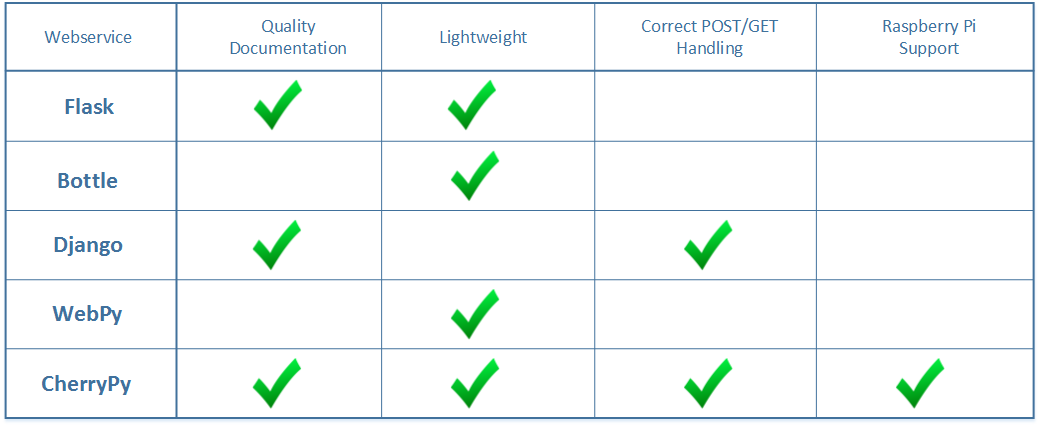
\includegraphics[scale=0.6]{Figures/webtable.png}
\caption{Comparison between five of the chosen webservices}
\label{fig:webtab}
\end{figure}

\textbf{CherryPy}
\paragraph{}
CherryPy is a minimalistic python object-oriented framework which focuses on flexibility and has a reliable HTTP/1.1-complient, WSGI thread
pooled web server. It requires a small amount of source code to run it, making it very useful to take the purpose of an \textit{Evaluator}. The \textit{Evaluator}
needs to be light in order to run either with multiple instances on a single server or run on a small devices like a Raspberry Pi.
\subsection{Genetic Programming Framework}
Genetic programming frameworks didn't have as many choices as RESTful web services however there was the option of implementing one.  Pyevolve\cite{pyevolve}, pystep\cite{pystep}, pygene\cite{pygene} and DEAP\cite{deap} were 
the only choices for genetic programming frameworks in python. None of them was minimalistic and simple enough, however implementing a genetic programming framework seemed a more complicated task
that could slow down the project and its final result. The most common and supported one was
the DEAP framework that also had really good documentation, tutorials and examples making it the correct choice. However as a future development option for the project
remains creating a genetic programming framework related to the project.
\subsection{Code Inspection and Generation}
Code inspection and generation was needed in order to achieve automation. Code inspection is used to extract source and information from live objects (e.g. modules, classes, methods, functions, tracebacks, 
frame objects, code objects). Generation is used to create new code objects and execute them in the scope of the program.
For inspecting code the best solution was the \textit{inspect} library which provided a way to extract source and other parameters from functions. It is a library that comes with python, 
has great documentation, examples and tutorials which proved positive for the speed of development.
\paragraph{}
Among one of the problems with using DEAP was it didn't support conversion between individuals and python source code or AST ( Abstract Syntax Tree). Representing an individual as raw code or an AST meant that 
the evaluating web service can be simplified even more. Using AST was very compatible with the way individuals are represented in genetic programming and it was more
robust and safe way of doing code generation rather than using raw string. However the more simple choice = raw strings, was selected due to pressure of time.  This suggested the idea of an open source contribution to the DEAP framework
 for generating python source 
and AST for a DEAP individuals.
\subsection{Graphical User Interface and XML}
Since the system is working with many parameters configuring them needed an abstraction. Using XML files for parsing parameters was the choice of abstraction. A parser was created
using lxml\cite{lxml} and connected with the graphical user interface.
Graphical user interface was the next step in project simplification. Its role was to generate XML files for the user with the ease of controlling all the parameters needed.
For creating GUI in python there are several good choices Tkinter, PyQT, wxPython. I've had prior experience with Tkinter and I wasn't excited about working with it again. It looked
much more complex compared to the other two. In sites such as StackOverflow the community was supporting wxPython. An additional benefit to using wxPython was the fact that there were a
lot of good tools for generating layout. However, my previous experience with GUI frameworks like Swing and its similarities with wxPython, gave me the advantage of understanding wxPython
quickly and writing a decent GUI in no time. In the end I didn't use any of the layout generating tools like wxGlade, wxDesigner or DialogBlocks because learning to use them was going to
cost almost the same time as learning wxPython.
\paragraph{}
\textbf{wxPython}
\paragraph{}
WxPython follows the standard graphical library design pattern -MVC (Model View Controller).
This design is focused on separation of concerns making it perfect for building a GUI for creation of XML files. The model or the 
data is the configuration parameters used, the view is the wxPython's frame and interface and the controller is the XML parser making use of data.
\paragraph{}
The library provides an easy to understand and use API. The main component is a frame, each secondary component like a pane, button or a menubar
is added to it. The framework uses different types of sizers to organize the components in the frame. To create more complex layouts
sizers can be stacked. WxPython has a large number of pre-set and easy to configure dialogue boxes for almost any case that might be needed.
More complex components were later created because of framework's versatility and modularity.